\documentclass[utf8, a4paper]{beamer}
\usepackage[french] {babel}
\usepackage[T1]      {fontenc}

\usepackage{amsmath, amsfonts, graphicx}
\usepackage{bibunits, tikz}

\usetheme{progressbar}
\graphicspath{{images/}}

\setbeamersize
  {text margin left=1em, text margin right=1em}

%\begin{itemize}
%	\item Brought to you by Cédric Mauclair
%	\item Please let me know about improvements!
%	\item Inspiration: \url{http://www.shawnlankton.com}... (in code)
%\end{itemize}

\title
  [Short Title]
  {Trajectory Optimization for Completion Time Minimization in UAV-Enabled Multicasting}

\author
  [Toto]
  {Riri\quad Fifi\quad Loulou }

\date
  {December 4, 2018}

\institute
  {ENAC}

\begin{document}

\maketitle

\begin{frame}{Plan}

  \tableofcontents

\end{frame}

\section {Introduction}

\begin{frame}
  {Introduction}
The rest of this paper is organized as follows. Section II
presents the system model and problem formulation. In
Section III, the lower bound of the file recovery probability
is derived, based on which the optimization problem is
reformulated. In Section IV, the proposed UAV trajectory
designs are presented. Section V provides the numerical
results, and finally we conclude the paper in Section VI.
  Things in a Bulleted List\pause

  \begin{enumerate}
  \item Bullets that
    \begin{enumerate}
    \item one
    \item two
    \end{enumerate}\pause
  \item Come up
    \begin{enumerate}
    \item one
    \item \emph{two} and three
    \end{enumerate}\pause
  \item One by one
    \begin{enumerate}
    \item one
    \item two
    \end{enumerate}
  \end{enumerate}
\end{frame}


\section{Modélisation du système et du problème}
\subsection{Equations}

\begin{frame}
{Equations}

Equations are easy
\begin{itemize}
	\item Just copy/paste equations\pause
	\item From the paper!
	\begin{equation*}
	\textbf{p}^* = \underset{\textbf{p}}{\arg\!\min}~\sum_{\textbf{x}}\left[ I(\textbf{W}(\textbf{x};\textbf{p})) - T(\textbf{x}) \right]^2
	\end{equation*}
\end{itemize}
\end{frame}

\section{Borne inférieure de la probabilité de bonne réception du fichier et reformulation du problème}



\begin{frame}{Equations}

  Equations are easy
  \begin{itemize}
  \item Just copy/paste equations\pause
  \item From the paper!
    \begin{equation*}
      \textbf{p}^* = \underset{\textbf{p}}{\arg\!\min}~\sum_{\textbf{x}}\left[ I(\textbf{W}(\textbf{x};\textbf{p})) - T(\textbf{x}) \right]^2
    \end{equation*}
  \end{itemize}
\end{frame}

\section{Proposition de conception de trajectoire}


\begin{frame}{Pictures}

  \begin{figure}[t]
    \centering
    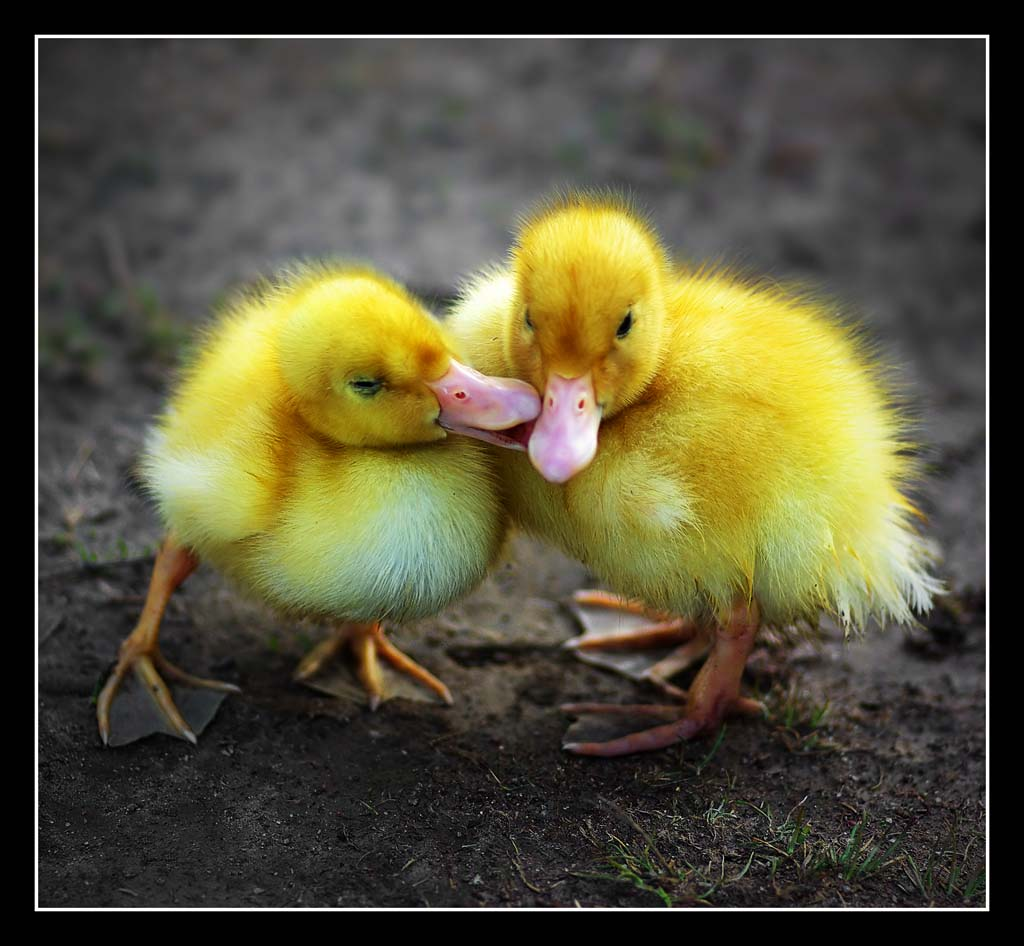
\includegraphics[height=\dimexpr11\textheight/16\relax]{ducks}
    \caption{Kissing ducks}
  \end{figure}
\end{frame}

\section{Résultats numériques}
\begin{frame}{A Movie}

  \begin{block} {Some block}

    \begin{itemize}
    \item Movies only seem to work in Adobe Reader
    \item Movie file is not embedded, it must be on the computer
    \end{itemize}
  \end{block}

  \pause
  \begin{alertblock}
    {Some more block}

    Movies only seem to work in Adobe Reader\\
    Movie file is not embedded, it must be on the computer
  \end{alertblock}
  \pause

  \begin{exampleblock}{}
    Some text in here.

    \begin{itemize}[<+->]
    \item Movies only seem to work in Adobe Reader
    \item Movie file is not embedded, it must be on the computer and
      what happe with a very long item?
    \end{itemize}
  \end{exampleblock}
\end{frame}


\section
  {Conclusion}

\begin{bibunit}[plain]
\begin{frame}
  {Credits}
This paper studied the trajectory design problem for a
UAV-enabled multicasting system to minimize the mission
completion time, while ensuring that each GT is able to
successfully recover the file with a high target probability.
We first converted the formulated optimization problem into
a more tractable form based on the derived analytical lower
bound of the successful file recovery probability, so that its
complicated constraint for each GT is simplified to one on
its minimum connection time with the UAV. We showed that
the optimal UAV trajectory only needs to constitute connected
line segments, which can be determined by finding the optimal
set of waypoints and then the optimal speed over time along
the path connecting the waypoints. We proposed two practical
waypoints design schemes and applied the LP to find the
optimal traveling speed given waypoints
  \begin{itemize}
 \item
  \end{itemize}

  \nocite{ipsum}
  \bibliography{sujet1}

\end{frame}
\end{bibunit}

\begin{bibunit}[plain]
\begin{frame}
  {Questions}

  \nocite{lorem}
  \bibliography{demo}

\end{frame}
\end{bibunit}


\appendix[Appendices]

\begin{frame}
  \frametitle{First appendix}
\end{frame}

\begin{frame}
  \frametitle{Second appendix}
\end{frame}

\end{document}


